% GNUPLOT: LaTeX picture with Postscript
\begingroup
  \makeatletter
  \providecommand\color[2][]{%
    \GenericError{(gnuplot) \space\space\space\@spaces}{%
      Package color not loaded in conjunction with
      terminal option `colourtext'%
    }{See the gnuplot documentation for explanation.%
    }{Either use 'blacktext' in gnuplot or load the package
      color.sty in LaTeX.}%
    \renewcommand\color[2][]{}%
  }%
  \providecommand\includegraphics[2][]{%
    \GenericError{(gnuplot) \space\space\space\@spaces}{%
      Package graphicx or graphics not loaded%
    }{See the gnuplot documentation for explanation.%
    }{The gnuplot epslatex terminal needs graphicx.sty or graphics.sty.}%
    \renewcommand\includegraphics[2][]{}%
  }%
  \providecommand\rotatebox[2]{#2}%
  \@ifundefined{ifGPcolor}{%
    \newif\ifGPcolor
    \GPcolorfalse
  }{}%
  \@ifundefined{ifGPblacktext}{%
    \newif\ifGPblacktext
    \GPblacktexttrue
  }{}%
  % define a \g@addto@macro without @ in the name:
  \let\gplgaddtomacro\g@addto@macro
  % define empty templates for all commands taking text:
  \gdef\gplbacktext{}%
  \gdef\gplfronttext{}%
  \makeatother
  \ifGPblacktext
    % no textcolor at all
    \def\colorrgb#1{}%
    \def\colorgray#1{}%
  \else
    % gray or color?
    \ifGPcolor
      \def\colorrgb#1{\color[rgb]{#1}}%
      \def\colorgray#1{\color[gray]{#1}}%
      \expandafter\def\csname LTw\endcsname{\color{white}}%
      \expandafter\def\csname LTb\endcsname{\color{black}}%
      \expandafter\def\csname LTa\endcsname{\color{black}}%
      \expandafter\def\csname LT0\endcsname{\color[rgb]{1,0,0}}%
      \expandafter\def\csname LT1\endcsname{\color[rgb]{0,1,0}}%
      \expandafter\def\csname LT2\endcsname{\color[rgb]{0,0,1}}%
      \expandafter\def\csname LT3\endcsname{\color[rgb]{1,0,1}}%
      \expandafter\def\csname LT4\endcsname{\color[rgb]{0,1,1}}%
      \expandafter\def\csname LT5\endcsname{\color[rgb]{1,1,0}}%
      \expandafter\def\csname LT6\endcsname{\color[rgb]{0,0,0}}%
      \expandafter\def\csname LT7\endcsname{\color[rgb]{1,0.3,0}}%
      \expandafter\def\csname LT8\endcsname{\color[rgb]{0.5,0.5,0.5}}%
    \else
      % gray
      \def\colorrgb#1{\color{black}}%
      \def\colorgray#1{\color[gray]{#1}}%
      \expandafter\def\csname LTw\endcsname{\color{white}}%
      \expandafter\def\csname LTb\endcsname{\color{black}}%
      \expandafter\def\csname LTa\endcsname{\color{black}}%
      \expandafter\def\csname LT0\endcsname{\color{black}}%
      \expandafter\def\csname LT1\endcsname{\color{black}}%
      \expandafter\def\csname LT2\endcsname{\color{black}}%
      \expandafter\def\csname LT3\endcsname{\color{black}}%
      \expandafter\def\csname LT4\endcsname{\color{black}}%
      \expandafter\def\csname LT5\endcsname{\color{black}}%
      \expandafter\def\csname LT6\endcsname{\color{black}}%
      \expandafter\def\csname LT7\endcsname{\color{black}}%
      \expandafter\def\csname LT8\endcsname{\color{black}}%
    \fi
  \fi
  \setlength{\unitlength}{0.0500bp}%
  \begin{picture}(8502.00,11338.00)%
      \csname LTb\endcsname%
      \put(4251,11118){\makebox(0,0){\strut{}\textbf{Beispiel eines verrauschten Signals}}}%
    \gplgaddtomacro\gplbacktext{%
      \csname LTb\endcsname%
      \put(946,8116){\makebox(0,0)[r]{\strut{}-1.0}}%
      \put(946,8701){\makebox(0,0)[r]{\strut{}-0.5}}%
      \put(946,9287){\makebox(0,0)[r]{\strut{}0.0}}%
      \put(946,9872){\makebox(0,0)[r]{\strut{}0.5}}%
      \put(946,10457){\makebox(0,0)[r]{\strut{}1.0}}%
      \put(1078,7896){\makebox(0,0){\strut{}0.0}}%
      \put(3854,7896){\makebox(0,0){\strut{}0.1}}%
      \put(176,9286){\rotatebox{-270}{\makebox(0,0){\strut{}$U \ [V]$}}}%
      \put(2466,7566){\makebox(0,0){\strut{}$t \ [s]$}}%
      \put(2466,10787){\makebox(0,0){\strut{}Zeitverlauf Sinusschwingung}}%
    }%
    \gplgaddtomacro\gplfronttext{%
    }%
    \gplgaddtomacro\gplbacktext{%
      \csname LTb\endcsname%
      \put(5065,8116){\makebox(0,0)[r]{\strut{}0.0}}%
      \put(5065,8701){\makebox(0,0)[r]{\strut{}0.2}}%
      \put(5065,9287){\makebox(0,0)[r]{\strut{}0.4}}%
      \put(5065,9872){\makebox(0,0)[r]{\strut{}0.6}}%
      \put(5065,10457){\makebox(0,0)[r]{\strut{}0.8}}%
      \put(5197,7896){\makebox(0,0){\strut{}0}}%
      \put(8105,7896){\makebox(0,0){\strut{}1000}}%
      \put(4427,9286){\rotatebox{-270}{\makebox(0,0){\strut{}$F$}}}%
      \put(6651,7566){\makebox(0,0){\strut{}$f \ [Hz]$}}%
      \put(6651,10787){\makebox(0,0){\strut{}Frequenzspektrum Sinusschwingung}}%
    }%
    \gplgaddtomacro\gplfronttext{%
    }%
    \gplgaddtomacro\gplbacktext{%
      \csname LTb\endcsname%
      \put(946,4800){\makebox(0,0)[r]{\strut{}-0.2}}%
      \put(946,5581){\makebox(0,0)[r]{\strut{}0.0}}%
      \put(946,6361){\makebox(0,0)[r]{\strut{}0.2}}%
      \put(1078,4190){\makebox(0,0){\strut{}0.0}}%
      \put(3854,4190){\makebox(0,0){\strut{}0.1}}%
      \put(176,5580){\rotatebox{-270}{\makebox(0,0){\strut{}$U \ [V]$}}}%
      \put(2466,3860){\makebox(0,0){\strut{}$t \ [s]$}}%
      \put(2466,7081){\makebox(0,0){\strut{}Zeitverlauf Rauschen}}%
    }%
    \gplgaddtomacro\gplfronttext{%
    }%
    \gplgaddtomacro\gplbacktext{%
      \csname LTb\endcsname%
      \put(5197,4410){\makebox(0,0)[r]{\strut{}0.00}}%
      \put(5197,6751){\makebox(0,0)[r]{\strut{}0.01}}%
      \put(5329,4190){\makebox(0,0){\strut{}0}}%
      \put(8105,4190){\makebox(0,0){\strut{}1000}}%
      \put(4427,5580){\rotatebox{-270}{\makebox(0,0){\strut{}$F$}}}%
      \put(6717,3860){\makebox(0,0){\strut{}$f \ [Hz]$}}%
      \put(6717,7081){\makebox(0,0){\strut{}Frequenzspektrum Rauschen}}%
    }%
    \gplgaddtomacro\gplfronttext{%
    }%
    \gplgaddtomacro\gplbacktext{%
      \csname LTb\endcsname%
      \put(946,704){\makebox(0,0)[r]{\strut{}-0.3}}%
      \put(946,1875){\makebox(0,0)[r]{\strut{}0.0}}%
      \put(946,3046){\makebox(0,0)[r]{\strut{}0.3}}%
      \put(1078,484){\makebox(0,0){\strut{}0.0}}%
      \put(3854,484){\makebox(0,0){\strut{}0.1}}%
      \put(176,1875){\rotatebox{-270}{\makebox(0,0){\strut{}$U \ [V]$}}}%
      \put(2466,154){\makebox(0,0){\strut{}$t \ [s]$}}%
      \put(2466,3376){\makebox(0,0){\strut{}Zeitverlauf verrauschte Sinusschwingung}}%
    }%
    \gplgaddtomacro\gplfronttext{%
    }%
    \gplgaddtomacro\gplbacktext{%
      \csname LTb\endcsname%
      \put(5197,704){\makebox(0,0)[r]{\strut{}0.00}}%
      \put(5197,3046){\makebox(0,0)[r]{\strut{}0.05}}%
      \put(5329,484){\makebox(0,0){\strut{}0}}%
      \put(8105,484){\makebox(0,0){\strut{}1000}}%
      \put(4427,1875){\rotatebox{-270}{\makebox(0,0){\strut{}$F$}}}%
      \put(6717,154){\makebox(0,0){\strut{}$f \ [Hz]$}}%
      \put(6717,3376){\makebox(0,0){\strut{}Frequenzspektrum verrauschte Sinusschwingung}}%
    }%
    \gplgaddtomacro\gplfronttext{%
    }%
    \gplbacktext
    \put(0,0){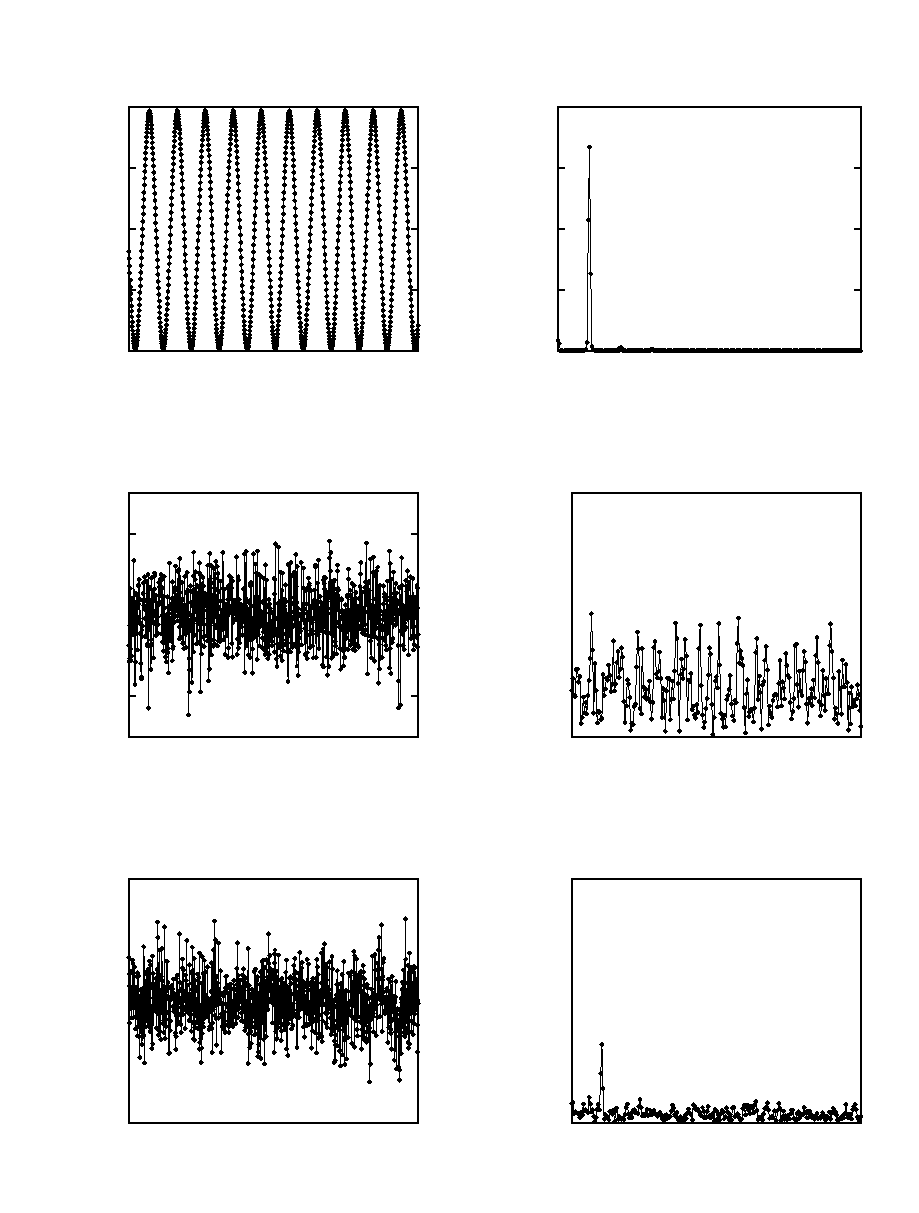
\includegraphics{3-sinus-noise}}%
    \gplfronttext
  \end{picture}%
\endgroup
